\chapter{基于深度强化学习的出行模式与时间选择方法}
\label{chp:float}

强化学习是一种通过迭代地改进策略来最大化累计奖励或回报的机器学习方法。在应用强化学习到具有马尔可夫属性的序列决策过程中,需要先构建一个马尔可夫决策过程,该过程定义了环境的演变,考虑到强化学习代理所采取的行动。强化学习代理通过行动探索和开发不断地与环境互动,根据当前状态 $s_t$ 进行行动。每次行动会使环境演变成一个新状态 $s_{t+1}$,并获得相应的奖励 $r_t$,反馈给代理以改善其决策逻辑。这个过程一直迭代,直到代理成功学习到一个能够最大化累计奖励的策略 $\pi$,也就是一个决策者。因此,强化学习的关键在于根据奖励不断迭代改进策略。

在本研究中,将每个出行者视为具有学习能力的智能实体,通过马尔可夫决策过程来建模每个出行者跨越多个连续日的交通出行行为。每个出行者能够选择的行动包括不同组合的出行方式和出发时间。最终由个人采取的行动 $a_t$ 决定了环境演变到的下一个状态 $s_{t+1}$。该状态应反映个人关于行程本身以及相关环境的最新知识。选择此行动所获得的奖励 $r_t$(与旅行成本相关)有助于改善个人的决策逻辑,这样个人就能逐渐学习到最优的行动策略,并最大化累计奖励。图\ref{RLintro}展示了在出行模式与时间选择问题背景下的强化学习中智能体与环境的交互示意图。

\begin{figure}[H]
  \centering
  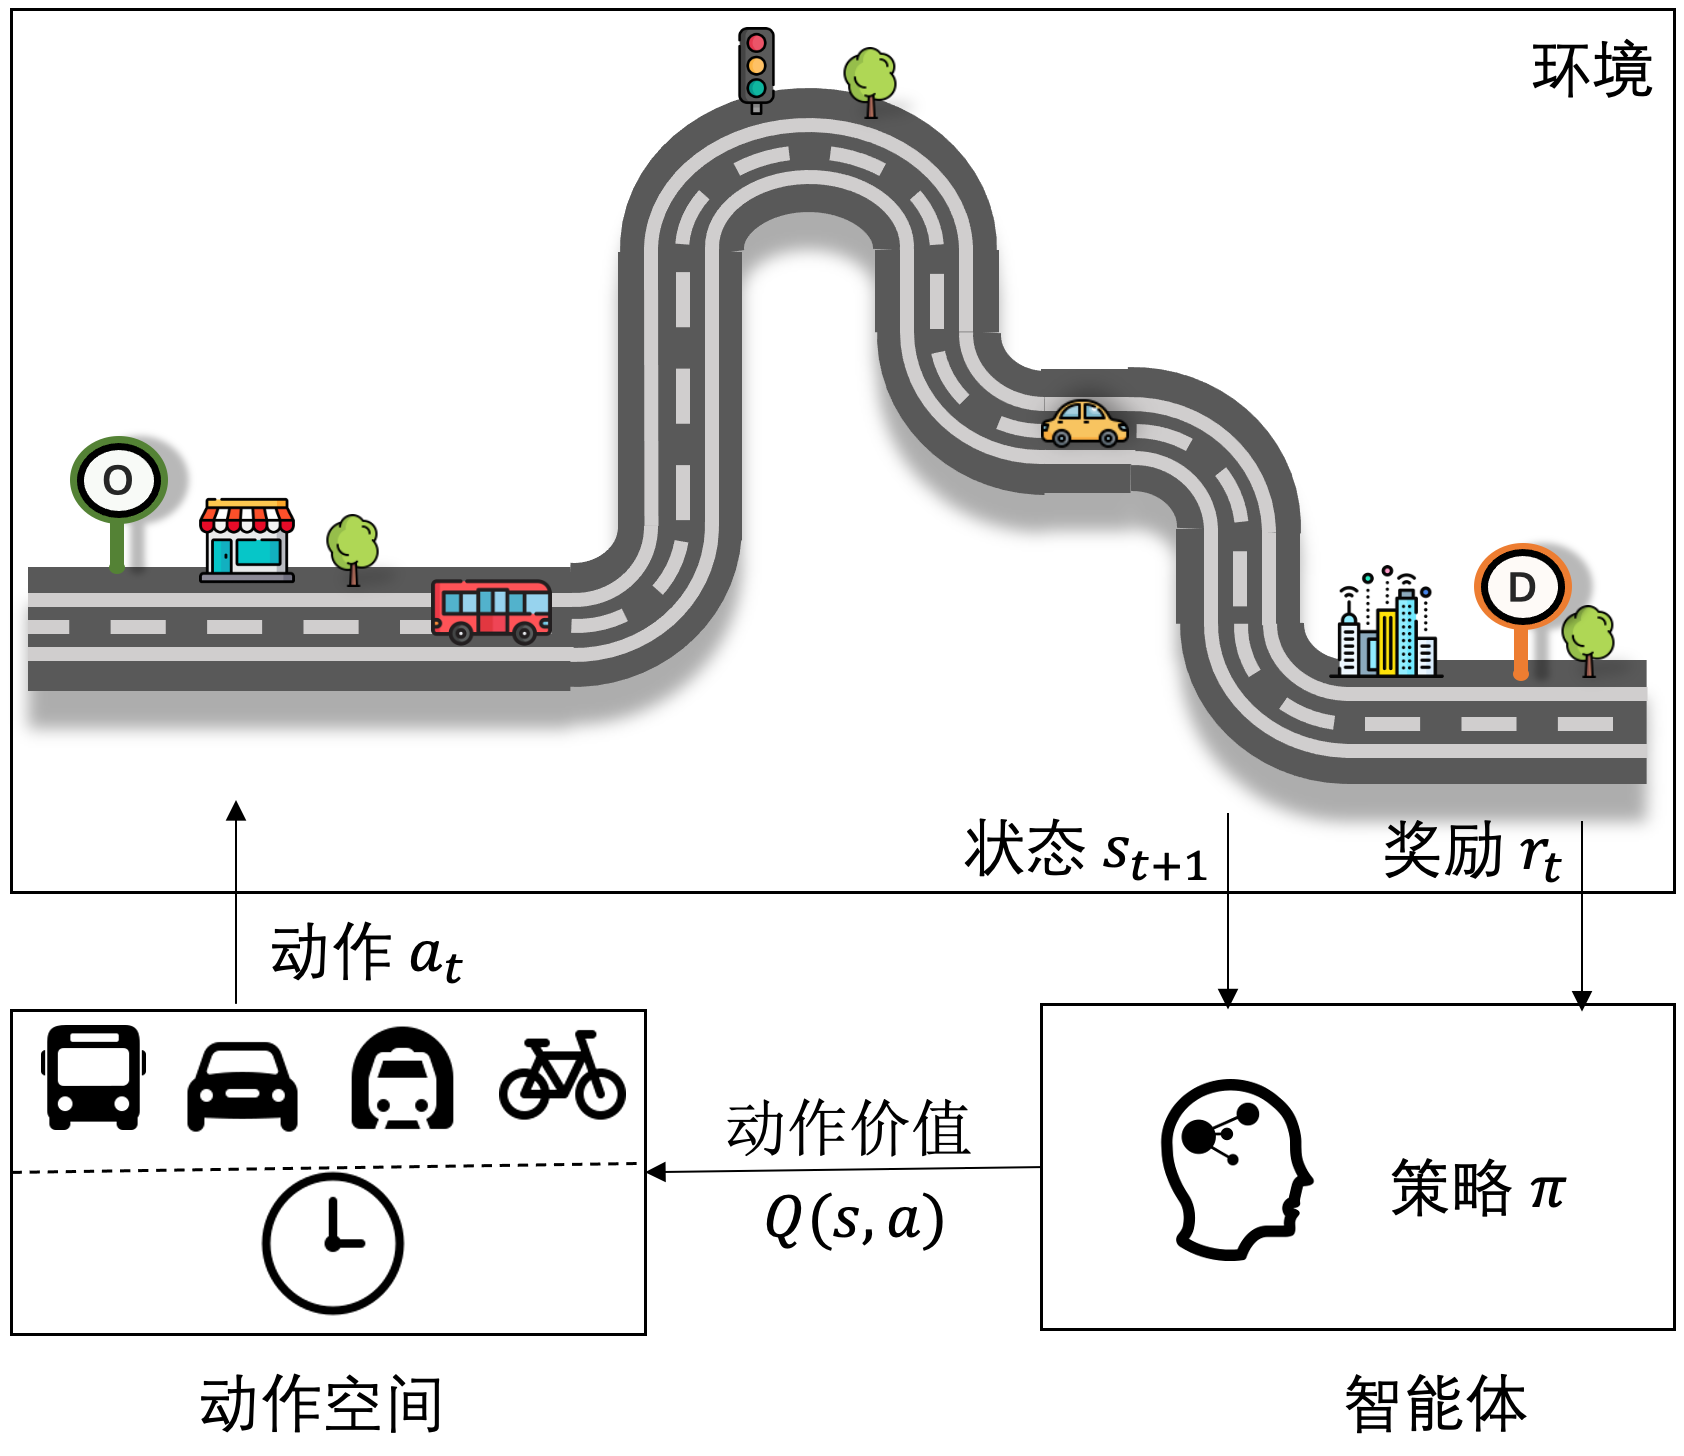
\includegraphics[width=.65\linewidth]{figures/content/RLintro.png}
  \caption{基于强化学习的出行模式与时间选择示意图}
  \label{RLintro}
\end{figure}

本章主要建立基于深度强化学习的出行模式与时间选择模型。首先,将使用马尔可夫决策过程框架来建模出行决策过程,包括定义状态空间、动作空间和奖励函数。然后,将介绍基于深度神经网络算法的出行模式和出发时间选择算法,并讨论如何设计合适的神经网络结构、选择超参数以及对模型进行优化和训练。最后,通过训练结果评估模型的性能。

\section{马尔可夫决策过程框架}
\label{sec:4_1}
马尔可夫决策决策过程是建模和优化出行模式和时间选择的先决条件。从数学角度来说,它是一个五元组$(S, A, P, R, \gamma)$,其中$S$表示状态空间,$A$表示动作空间,$P$表示状态转移概率,$R$表示奖励函数,$\gamma$为折扣因子。接下来,将进一步阐述如何构建和解决本文研究的特定问题下的马尔可夫决策决策过程。



\subsection{动作空间}

动作空间是强化学习中的一个关键概念。在建模动作空间时需考虑出行者的个性化特征。例如,不同出行者对于出行方式和出发时间的偏好不同,因此他们的动作空间也会不同。对此,可以引入个性化因素对动作空间进行建模。例如,可以考虑出行者的年龄、性别、职业、家庭状况等因素,进一步细化动作空间的描述,提高模型的预测能力和适应性。此外,动作空间的大小和粒度也会影响到模型的性能和可解释性。如果动作空间过大,模型的训练和预测会变得非常困难,同时也会增加模型的计算复杂度和存储空间需求。而如果动作空间过小,模型的表达能力就会受到限制,无法对真实情况进行有效建模。因此,需要在合理范围内对动作空间进行定义和限制,以平衡模型的性能和可解释性。在实际应用中,建模动作空间的过程也需要考虑到数据的可用性和质量。

在出行模式与时间选择中,动作空间包括出行方式和出发时间两个方面。在选择出发时间时,出行者需要考虑到交通拥堵、出行时间和其他因素对行程的影响。例如,在高峰期出发可能需要更长的旅行时间,而在非高峰期出发可能可以更快地到达目的地。因此,在建模动作空间时,需要综合考虑各种因素,以便在代理决策时提供准确的信息。

其中,出行模式的选择包含私家车、公共交通或自行车。在公共交通中,可以选择乘坐公交车或地铁,以及在公交地铁间的换乘,但是不考虑三种交通方式之间的换乘。这是因为在与多模式换乘中涉及到很多变量,比如停车地点、换乘时间等,考虑到乘客在选择时的不会多次更换交通模式的实际决策情况以及研究的复杂程度,本研究将不考虑不同模式之间的多次换乘行为。

对于出发时间,每个出行者都有一个初始或期望出发时间$t_0$。实际上,在早高峰出行时,出行者往往会考虑调整出发时间,以避免交通拥堵和延误。这种现象被称为“出行时间弹性”(travel time elasticity),指的是出行者在面对交通拥堵或不确定性时,可以调整出行时间以获得更好的出行体验或更高的效率。根据交通经济学的研究,出行时间弹性的大小受到许多因素的影响,包括个人时间成本、出行目的、所处的交通环境以及出行者的偏好等。因此,在出行模式和时间选择算法中,需要考虑出行时间弹性,以更准确地推荐出行模式和出发时间。在本文的出行模式与时间选择场景中,出发时间可以在一个有限的时间窗口$[t_{\min},t_{\max}]$内进行调整。这个时间窗口是由最早和最晚的出发时间$t_{\min}$和$t_{\max}$确定的。出发时间的调整是以离散间隔为单位进行的,而不是连续方式进行。在本文的出行模式与时间选择场景中,离散间隔的设置是为了将出发时间的选择问题转化为一个有限的状态空间的问题,从而可以应用深度强化学习算法进行求解。如果使用连续方式进行出发时间的调整,状态空间将是无限的,这将导致算法难以收敛并且计算复杂度较高。因此,将出发时间的调整以离散间隔为单位进行,可以有效地简化问题,并且使算法更易于实现和计算。

对于上述所提到的交通方式和出发时间,需要进行适当的编码以便于智能体在模型中进行操作。在本文中,采用离散化编码的方式,将交通方式和出发时间分别离散化为一组离散的选项。例如,对于交通方式,可以将私家车、公交车、地铁和自行车分别编码为$m_1$、$m_2$、$m_3$和$m_4$。对于出发时间,可以将$t_0$和时间窗口$[t_{\min},t_{\max}]$离散化为一组时间步长,例如每5分钟一步。这样,代理可以从一组离散的选项中进行选择,并决定最佳的出行方式和出发时间。动作空间的描述采用了向量的形式,$\bm{a}$包括交通方式$\tilde{m}$和出发时间$\tilde{t}$。交通方式可以是可用交通方式$m_{1},m_{2}, \ldots, m_{N}$中的任意一种,而出发时间必须在时间窗口$[t_{\min }, t_{\max }]$内。因此,动作空间可以表示为:
\begin{equation}
\bm{a}=\left[\begin{array}{c}
\tilde{m} \\
\tilde{t}
\end{array}\right]=\left[\begin{array}{c}
\text { 出行模式 } \\
\text { 出发时间 }
\end{array}\right]
\in\left[\begin{array}{c}
\left\{m_{1},m_{2}, \ldots, m_{N}\right\} \\
{\left[t_{\min }, t_{\max }\right]}
\end{array}\right]
\end{equation}

\subsection{状态空间}

状态空间是强化学习中非常重要的一个概念,它定义了智能体在决策时需要考虑的连续环境。在设计状态空间时,需要仔细考虑应用场景和问题的特征,以确保状态空间中包含的信息能够有效地指导代理的决策。同时,也需要注意状态空间的维度和大小,以便使智能体能够有效地处理状态,并且可以在有限的时间内完成状态的学习和更新。对于出行模式与时间选择的问题,状态空间被设计为不仅需要包含有关行程的最新信息,还包括智能体早期经验。这种状态空间设计在很大程度上类似于理性人类的决策机制,即从经验中学习。由于本研究的重点不在于经验选择建模而在于选择指导或推荐,因此将假设智能体能够充分感知环境,因此掌握行程的全部信息。

行程信息首先包括每种交通方式的旅行距离$L$和记忆旅行时间$\bar{T}$。前者是模式$m$的旅行距离,而后者是该模式$m$的平均经验旅行时间,这样可以利用经验和在交通随机性存在的情况下保持稳健性。作为行程信息的另外两个变量是初始出发时间$t_0$和出发时间差或偏移量$\Delta t$。将上述所有内容组合起来,得行程信息的状态向量${\bm{s}_\text{trip}^m}$:
\begin{equation}
\begin{aligned}
{\bm{s}_\text{trip}^m}=\left[\begin{array}{c}
L_m \\
{\bar{T}}_m \\
t_{0} \\
\Delta t
\end{array}\right]=&\left[\begin{array}{c}
\text { 出行距离 } \\
\text { 记忆行程时间 } \\
\text { 初始出发时间 } \\
\text { 出发时间差}
\end{array}\right]
\end{aligned}\label{equation:trip}
\end{equation}

环境信息基本上包括有助于不同交通方式旅行成本的因素。对于公共交通,考虑到两个因素,即可达性和票价。在这里,我们将可达性$p$定义为完成行程的第一和最后一段所需的总步行距离:

\begin{equation}
p=d_{\text{origin}}+d_{\text{destination}}
\end{equation}

其中$d_{\text{origin}}$和$d_{\text{destination}}$分别是从最近的公交车站或地铁站到起点和终点的步行距离。公共交通票价是必须支付的使用该服务的货币成本。对于私家车,我们考虑燃油价格作为影响因素,并将其放在状态中。因此,特定于环境信息的状态向量如下所示:

\begin{equation}
\begin{aligned}
\bm{s}_\text{environment}=\left[\begin{array}{c}
p \\
f \\
o 
\end{array}\right]=\left[\begin{array}{c}
\text { 可达性} \\
\text { 票价 }\\
\text { 燃油价格 }
\end{array}\right]
\end{aligned}\label{equation:env}
\end{equation}

为了将用户的时间价值纳入状态空间,将再添加一个状态向量来代表用户的偏好,并使用这个变量来调整不同状态下关联的时间价值。例如,对于高收入用户而言建议出行时间较长的状态造成更高的时间价值,因为这些用户可能有能力支付更昂贵但更快的交通方式。另一方面,对于低收入用户,时间价值会更低。基于此,我们提出的深度强化学习算法将学习考虑用户的收入水平来推荐旅行方式,并在用户特定的需求和偏好上权衡旅行时间和成本,从而做出适当的建议。
\begin{equation}
\begin{aligned}
\bm{s}_\text{VOT}=\left[\begin{array}{c}
\alpha
\end{array}\right]=\left[\begin{array}{c}
\text {时间价值} 
\end{array}\right]
\end{aligned}\label{equation:VOT}
\end{equation}

将式\ref{equation:trip}、式\ref{equation:env}与式\ref{equation:VOT}相结合,可以得到在完全信息假设下的完整状态空间。

实际人类在做选择时,通常无法获取所有的状态信息。因此,在模拟人类的选择行为,需要建立部分信息的状态空间向量。通过将某些状态变量排除在外,可以简化问题并减少计算复杂度。然而,这也会影响算法的性能和准确性,因为所选取的状态变量可能无法完全描述真实的状态。

实际上,在进行决策和选择时,人类通常无法获取所有的状态信息。这种现象在现实生活中尤为明显,因为面临许多复杂且不确定的情况。因此,在模拟人类的决策行为时,需要建立一个基于部分信息的状态空间向量,在众多可能的状态变量中挑选一部分来构建模型。通过将某些状态变量排除在外,可以简化问题并降低计算复杂度,从而加快求解速度和提高算法的效率。为了平衡问题的简化程度与保持准确性之间的关系,研究人员需要在选择状态变量时做出权衡。这通常涉及到对问题的深入理解和多次尝试。在实际应用中,可以通过逐步增加或减少状态变量的数量来调整算法的性能和准确性,以找到最适合特定问题的状态空间表示。然而,这种简化往往需要在算法的性能和准确性方面付出一定代价。由于所选取的状态变量可能无法充分描述真实的状态,这可能导致算法在某些情况下无法做出最佳决策。

\begin{equation}
\begin{aligned}
\bm{s}_\text{reduced}=\left[\begin{array}{c}
\bar{T} \\
t_{0} \\
\Delta t
\end{array}\right]=&\left[\begin{array}{c}
\text {记忆行程时间} \\
\text {初始出发时间} \\
\text {出发时间差}
\end{array}\right]
\end{aligned}\label{equation:obs}
\end{equation}



\subsection{奖励函数}
\label{subsection:reward}
在强化学习中,智能体的目标是通过最大化长期奖励来学习最优的决策规则。通过奖励函数,智能体可以计算每个动作对于实现这个目标的预期收益。在本文的研究中,奖励函数可以参考旅行效用函数,旨在最小化总旅行费用。智能体将根据预期的长期奖励来选择动作,以便在未来的交互中最大化收益。在第i步获得的奖励计算公式如下:

\begin{equation}
r_{i}=\frac{E_{1}-C_{m}^{i}}{E_{2}},\label{reward function}
\end{equation}

其中,$C_m^i$ 是交通方式$m$的总旅行费用,$E_1$ 和 $E_2$ 是映射和缩放成本到奖励的两个常数。总旅行费用又可以分解为三个部分,即总旅行时间$T_m^i$、行程延误$\delta(t^i)$ 和其他与旅行相关的成本$F_m^i$:

\begin{equation}
C_{m}^{i}=\alpha T_{m}^{i}+\delta\left(t^{i}\right)+F_{m}^{i},\label{costfunction}
\end{equation}

其中,$\alpha$ 是时间的价值。这个公式描述了在一个旅行过程中,成本是如何被划分的。智能体可以通过调整其动作来优化它所接收到的奖励,并在行程中实现更好的效用。

只考虑总旅行时间的问题往往会忽略实际到达时间。也就是说,尽管总的旅行时间很短,但到达时间可能与理想的时间相差甚远。因此,在成本计算中引入了计划延迟惩罚\cite{small1982scheduling}。假设每个人都有一个期望的到达时间,早到和晚到都会产生一个所谓的日程延误成本。当实际到达时间偏离期望时间时,计划延迟成本会以线性方式增长。从数学上讲,它表示为:。
\begin{equation}
\delta(t^i)= 
\begin{cases}\beta\left(t+T_{m}-t_\text{d}\right) & \text { if\quad } t+T_{m}-t_\text {d}<0, \\ 
0 & \text { if\quad } t+T_{m}-t_\text {d}=0, \\ 
\gamma\left(t_\text {d}-t-T_{m}\right) & \text { if\quad } t+T_{m}-t_\text {d}>0,
\end{cases}
\end{equation}

其中,$\beta$和$\gamma$分别是早到和晚到的行程延误时间价值,$t_\text{d}$是期望到达时间。通过考虑行程延误成本,可以更准确地评估各种出行方式的效用。

除此之外,其他的与出行相关的费用主要是指汽车的燃料费用和公共交通的票价。对于私家车来说,燃料费用是与行驶距离成正比的,而对于公共交通来说,则是根据具体的交通工具的票价。因此,其他出行相关费用可以表示为公式:
\begin{equation}
F_{m}^i= 
\begin{cases}
L_\text{car} \cdot o  & \text { if\quad  } m=\text { 私家车 }, \\ 
f  & \text { if\quad  } m=\text { 公共交通 }, \\ 
0   &  \text { if\quad } m=\text {自行车}
\end{cases}
\end{equation} 

其中,$f$可以表示为:

\begin{equation}
f=\mathbb{I}(\text { bus }) \cdot f_{\text {bus }}+\mathbb{I}(\text { subway }) \cdot f_{\text {subway }},
\end{equation}

这里的$\mathbb{I}(\cdot)$是一个指示函数,当选择的交通工具是公共汽车或地铁时,它返回1,否则返回0。公交车费用$f_{\text {bus }}$是固定的,而地铁费用$f_{\text {subway} }$则随着行驶距离的增加而增加。这些费用可以用于计算奖励函数中的其他出行相关成本项。

\section{基于深度Q网络算法的模式与出发时间选择算法}
\label{sec:4_2}

本文采用无模型基于动作的深度强化学习方法深度Q网络作为基础算法解决出行模式与时间选择问题。它学习与MDP相关的状态动作值,基于此隐含地推导出最优策略,即始终选择导致最大状态动作值的动作。根据式\ref{eq:2_5}与式\ref{eq:2_6}可知,它使用神经网络来近似最优状态动作值函数,从而将传统的Q-learning应用于高维或连续空间问题。

为了设计一个优秀的DQN算法,本节需要对神经网络结构进行设计,并对超参数进行选择和标定,然后对模型进行优化。神经网络结构设计应考虑输入和输出的特征,并充分考虑网络的深度和宽度。超参数包括学习率、批量大小、折扣因子和经验回放的容量。优化算法包括随机梯度下降、Adam和RMSProp等。通过选择适当的超参数和优化算法,可以提高DQN算法的收敛速度和性能。

\subsection{神经网络结构设计}


神经网络在强化学习中扮演着重要的角色,它可以作为函数逼近器来估计Q值函数,从而得到最优的策略。在DQN算法中,神经网络被用来近似状态-动作值函数,因此它的结构对算法的性能有着很大的影响。在DQN算法中的神经网络结构设计可以通过以下步骤进行:

1.确定输入和输出层的维度。神经网络的输入层节点通常接收标量值,每个输入节点代表输入数据中的一个特征,输出层的输出数据同理。当有多个特征时,输入层会有多个节点,每个节点对应一个特征。在本文的研究中,输入层的维度应该与状态向量的维度相同,而输出层的维度应该等于动作的数量。

2.选择合适的隐藏层数和节点数。神经网络的隐藏层节点数量和层数决定了网络的复杂性和表示能力。一个具有更多节点和层数的网络可能具有更强大的表示能力,但也可能导致过拟合,特别是在训练数据有限的情况下。相反,一个具有较少节点和层数的网络可能会降低过拟合的风险,但也可能导致模型的表达能力不足,从而导致欠拟合。在本研究的神经网络设计中,选择32、64、64这些值作为隐藏层的节点数量,这些值在实践中能够提供一个合理的平衡,既不会导致过拟合,也不会导致欠拟合。

3.选择适当的激活函数。激活函数对神经网络的性能有着重要的影响。在本文的深度Q网络中,神经网络使用ReLU作为激活函数(参考式\ref{eq:2_16})。ReLU函数的优点是计算简单,同时能够引入非线性特性。在许多深度学习任务中,ReLU激活函数表现良好,因此在DQN中也是一个常用的选择。

4.选择适当的优化器和损失函数。在训练过程中,将使用经验回放的技术来解决深度Q网络算法中的样本问题。通过将每个状态-动作转换存储在一个固定大小的缓存器中,使模型可以从以前的经验中学习。这种方法允许从整个经验集合中随机抽取样本进行训练,以减少梯度下降的样本相关性,并增加学习的稳定性。在优化深度Q网络算法时,使用均方误差损失函数(参考式\ref{eq:2_18})作为优化目标,其中$y_i$是目标Q值,可以通过式\ref{eq:2_6}计算得到。最后,使用优化器(如Adam)来调整神经网络的权重,以最小化损失函数。

图\ref{neuralnet}是本文深度Q网络中的神经网络结构示意图。在代码实现中,使用PyTorch框架来定义神经网络。在DQN类的初始化函数中,定义了前馈神经网络的结构。它包括四个线性层,分别包含32,64,64和n个节点,其中n是动作的数量。这个结构相对简单,在实际应用中已经被证明可以取得不错的效果。

\begin{figure}[H]
  \centering
  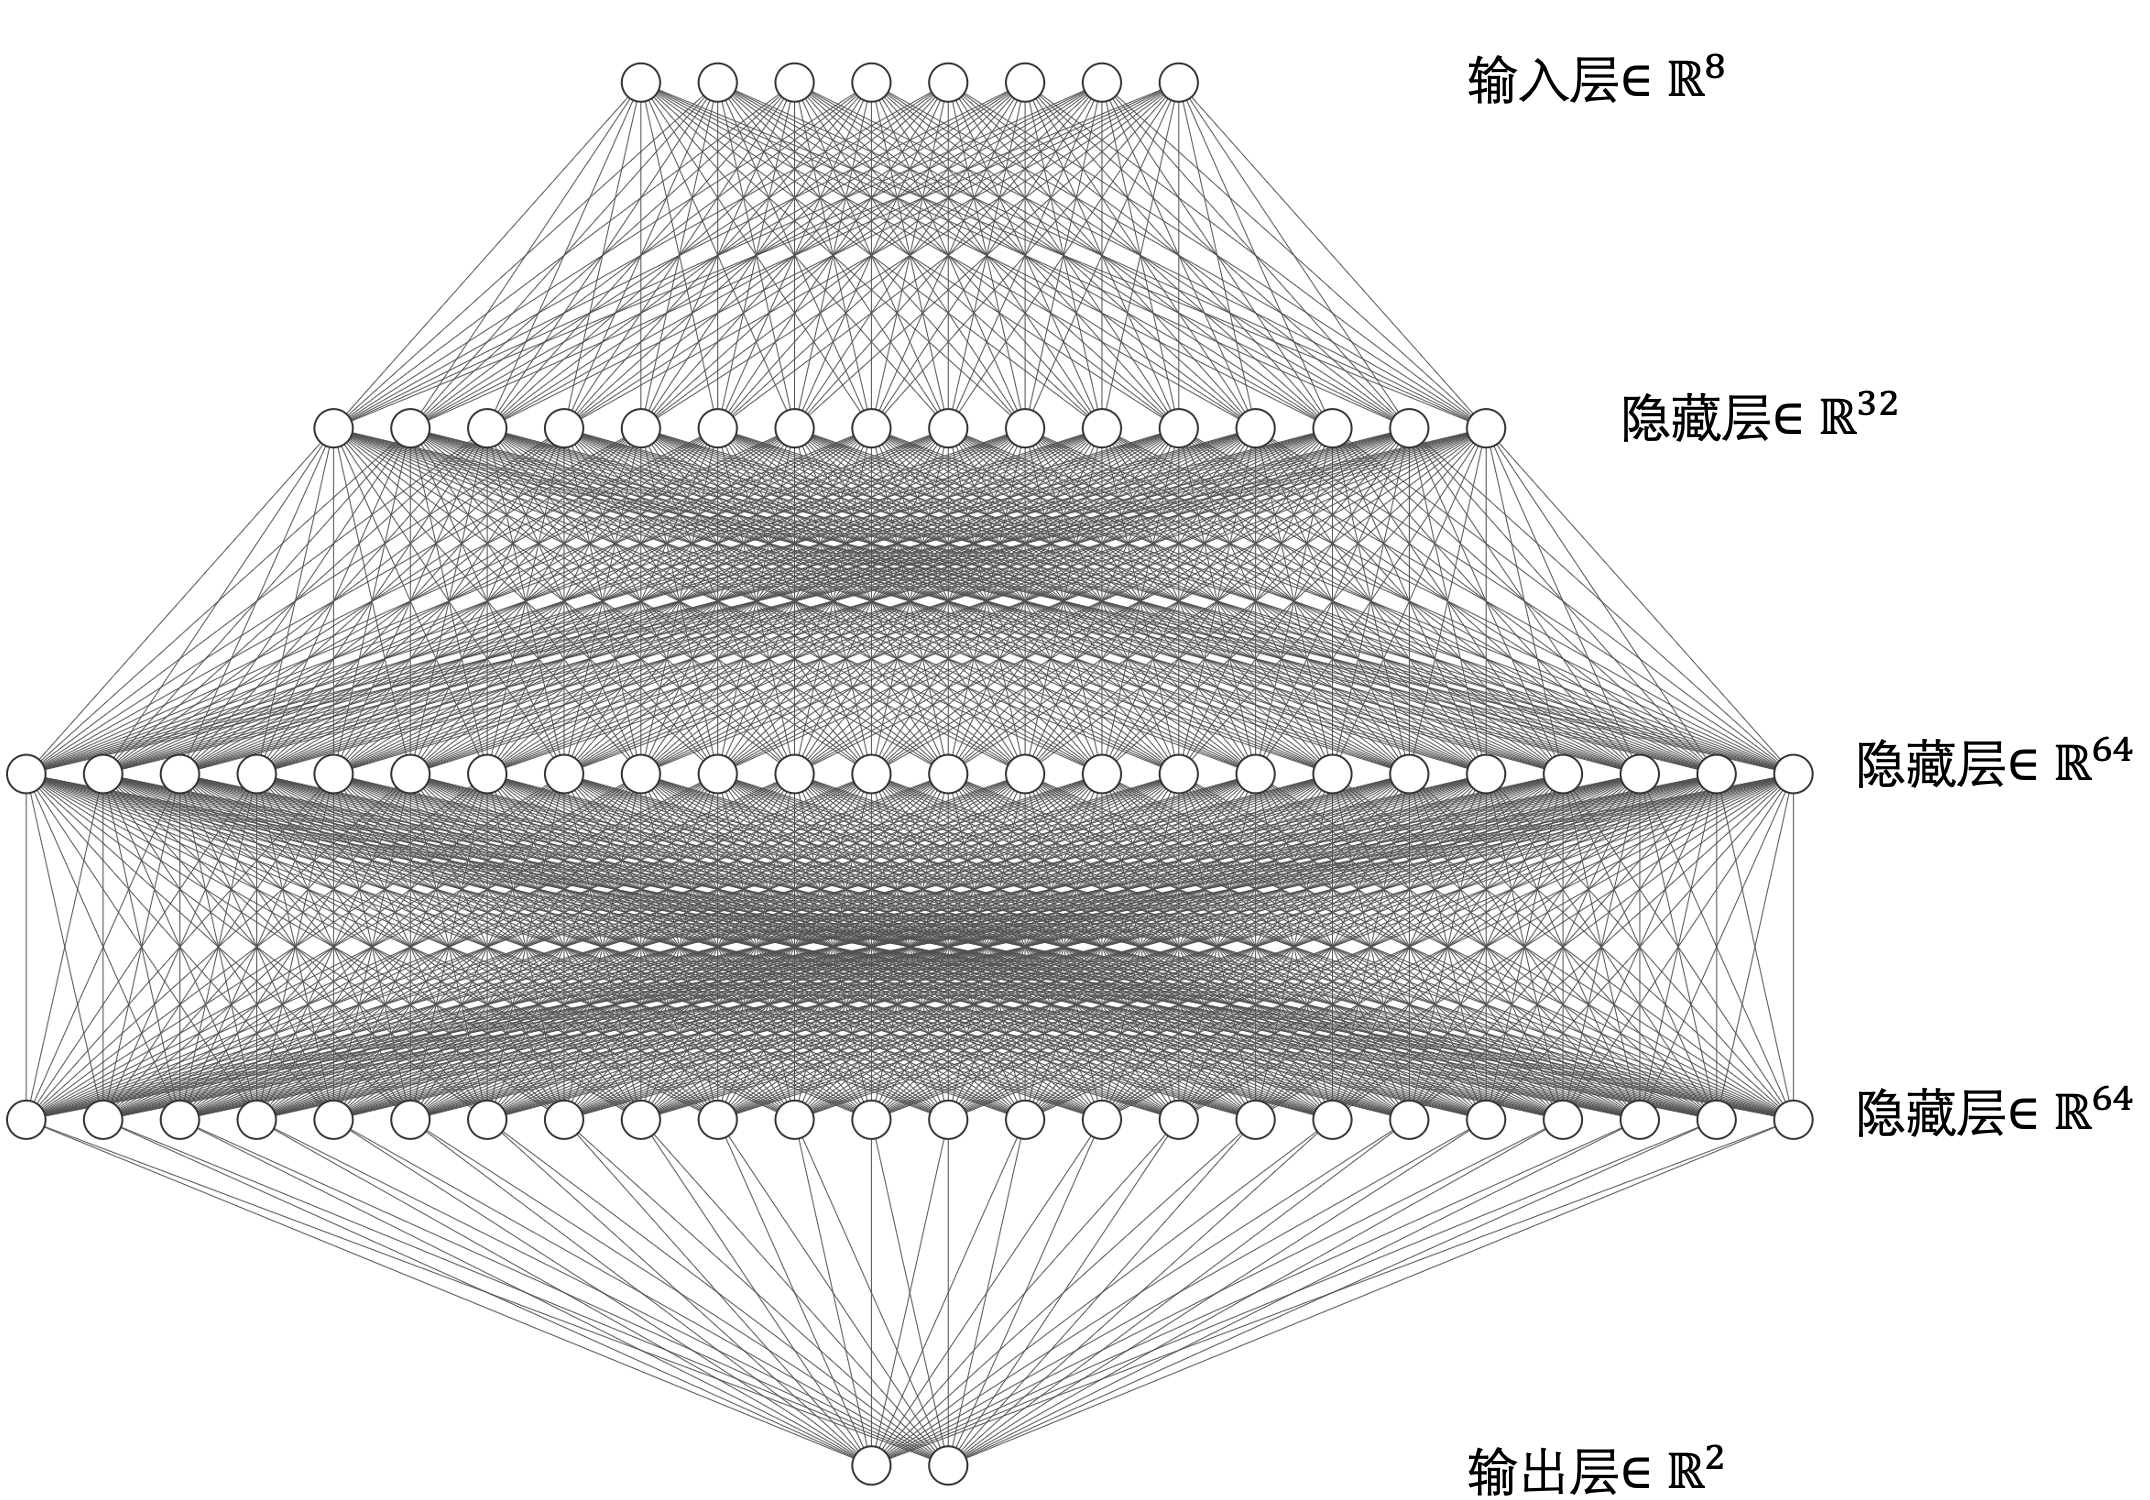
\includegraphics[width=.75\linewidth]{figures/content/neuralnet.png}
  \caption{神经网络结构示意图}
  \label{neuralnet}
\end{figure}




\subsection{超参数的选择}

超参数是在训练过程中固定不变的参数,它们对模型的性能和训练速度有很大影响。合适的超参数选择对于训练一个高效且鲁棒的模型至关重要。优化器的学习率等超参数的选择和标定也会对DQN算法的性能有很大的影响。因此,需要进行仔细的超参数调优,以找到最优的超参数组合,以提高DQN算法的收敛速度和性能。可以将不同超参数在深度Q网络中的作用将其分为四大类:学习与优化相关参数、经验回放相关参数、神经网络结构与同步相关参数和探索与利用相关参数。

学习与优化相关参数主要负责控制神经网络的学习过程,包括奖励折扣、学习速率和每次权重更新的样本数量。这些参数可以影响模型收敛速度和学到的策略质量。为了限制模型训练的时间和资源消耗,通常也会设置最大训练轮数,根据实际需求和计算资源,可以调整这个参数来平衡训练时间和模型性能。学习与优化相关参数包括GAMMA,BATCH\_SIZE,LEARNING\_RATE和MAX\_EPISODE。

GAMMA:折扣因子用于调整未来奖励的重要性。较高的值表示更关注未来的回报,而较低的值表示更关注短期回报。在本实验中,选择了0.99的折扣因子,以平衡短期和长期回报的关注度。

BATCH\_SIZE:每个训练步骤中使用的样本数。较大的批量大小可能会导致梯度更新更稳定,但同时也会增加计算成本。选择了5作为批量大小,以在计算效率和梯度稳定性之间取得平衡。

LEARNING\_RATE:模型在训练过程中更新权重的速度。较大的学习速率可能会导致模型收敛得更快,但也可能导致不稳定的训练过程。较小的学习速率可能会使训练过程更稳定,但需要更长的时间才能收敛。选择了1e-4作为学习速率,以在收敛速度和训练稳定性之间取得平衡。

MAX\_EPISODE:最大的训练轮数,用于限制训练时间。在实际应用中,训练时间可能受到硬件和计算资源的限制。我们选择了800作为最大训练轮数,以在保证模型性能和限制训练时间之间达到平衡。

经验回放是深度Q网络算法的一个关键组成部分,可以有效地降低数据相关性、提高样本利用率,从而加速学习过程。这类参数主要调整回放缓冲区的容量和在开始训练前填充缓冲区的样本数量,以确保训练过程中有足够的经验样本可以使用。经验回放相关参数包括REPLAY\_SIZE和REPLAY\_START\_SIZE。

REPLAY\_SIZE:回放缓冲区的最大容量。回放缓冲区用于存储经验样本,以便在训练过程中进行随机抽样。较大的回放缓冲区可以提高样本的多样性,但也会增加内存计算压力。经过多次实验测试后,最终选择了40作为回放缓冲区大小。

REPLAY\_START\_SIZE:开始训练前等待填充回放缓冲区的帧数。这个参数确保在训练开始时,回放缓冲区已经存储了足够的样本。选择40作为开始训练前填充回放缓冲区的帧数,以确保有足够的样本用于训练。

深度Q网络算法使用了两个相同结构的神经网络,一个用于训练,另一个作为目标网络计算目标值。这类参数主要负责控制训练网络和目标网络之间权重同步的频率。同步过程可以保证目标网络的稳定性,从而提高训练的稳定性。神经网络结构与同步相关参数包括SYNC\_TARGET\_FRAMES。

SYNC\_TARGET\_FRAMES:将模型权重从训练模型同步到目标模型的频率。定期将训练模型的权重同步到目标模型有助于提高训练过程的稳定性。经过多次实验测试后,选择了5作为同步频率,以在训练速度和稳定性之间达到平衡。

深度Q网络算法通过$\varepsilon$-greedy策略平衡探索(尝试新动作)和利用(采用当前最优策略)。这类参数主要用于调整探索程度,包括ε值的初始值、最终值以及从初始值到最终值所需的帧数。合适的探索与利用平衡有助于模型找到全局最优策略。探索与利用相关参数包括EPSILON\_START、EPSILON\_FINAL和EPSILON\_DECAY\_LAST\_FRAME。

EPSILON\_START:$\varepsilon$-greedy策略中的初始$\varepsilon$值。较高的初始$\varepsilon$值意味着在训练初期,智能体更倾向于探索环境而非利用已知的策略。选择1.0作为初始$\varepsilon$值,以鼓励智能体在训练初期进行充分的探索。

EPSILON\_FINAL:$\varepsilon$-greedy策略中的最终$\varepsilon$值。较低的最终$\varepsilon$值表示在训练后期,智能体更倾向于利用已知的策略而非进行探索。选择0.01作为最终$\varepsilon$值,以在训练后期降低探索频率并优化已知策略。

EPSILON\_DECAY\_LAST\_FRAME:$\varepsilon$值从初始值到最终值所需的帧数。较快的衰减速率可能会导致智能体在训练初期就过于关注已知策略,而较慢的衰减速率可能会导致智能体在训练过程中持续进行过多的探索,最终选择800作为衰减帧数。

表\ref{demand_inf}列出了经过测试与参考后确定的在深度Q网络中使用的超参数及其取值。
\renewcommand{\arraystretch}{1.2} % 使表格行间距加大1.5倍
\begin{table}[htbp]
\centering
\caption{参数的取值与描述}
\label{demand_inf}
\begin{tabular}{ccc}
\toprule
参数 & 取值 & 描述       \\
\midrule
GAMMA & 0.99 & 未来奖励的折扣因子 \\ 
BATCH\_SIZE & 5 & 每个训练步骤中使用的样本数 \\ 
REPLAY\_SIZE & 40 & 回放缓冲区的最大容量 \\ 
LEARNING\_RATE & 10$^{-4}$ & 模型在训练过程中更新权重的速度 \\ 
SYNC\_TARGET\_FRAMES & 5 & 将模型权重从训练模型同步到目标模型的频率 \\ 
REPLAY\_START\_SIZE & 40 & 开始训练前等待填充回放缓冲区的帧数 \\ 
EPSILON\_START & 1.0 & $\varepsilon$-greedy策略中的初始$\varepsilon$值 \\ 
EPSILON\_FINAL & 0.01 & $\varepsilon$-greedy策略中的最终$\varepsilon$值 \\ 
EPSILON\_DECAY\_LAST\_FRAME & 600 & $\varepsilon$值从初始值到最终值所需的帧数 \\ 
MAX\_EPISODE & 800 & 最大的训练轮数,用于限制训练时间 \\ 

\bottomrule
\end{tabular}
\end{table}



\subsection{模型的优化}

为了提高本研究中深度强化学习模型的性能,引入经验回放的技术。经验回放是一种重要的优化技术,它解决了DQN算法中的样本相关性问题。在传统的在线学习中,神经网络每次只更新一个样本的参数,因此相邻样本的训练数据之间存在强相关性,容易导致模型的过拟合。经验回放的核心思想是将所有样本存储到经验池中,并从中随机采样一批样本进行训练。这样可以打破样本之间的相关性,减少过拟合的风险,提高模型的泛化能力。

图\ref{reply}展示了经验回放缓冲区和目标网络的深度Q网络的工作流程。图中描绘了状态输入到主网络和目标网络的过程,以及如何将经验元组存储到经验回放缓冲区中。同时,从缓冲区中随机抽样的经验被用于计算损失并更新主网络。此外,通过某种策略(例如,每隔固定步数)更新目标网络,从而提高模型的稳定性。

\begin{figure}[H]
  \centering
  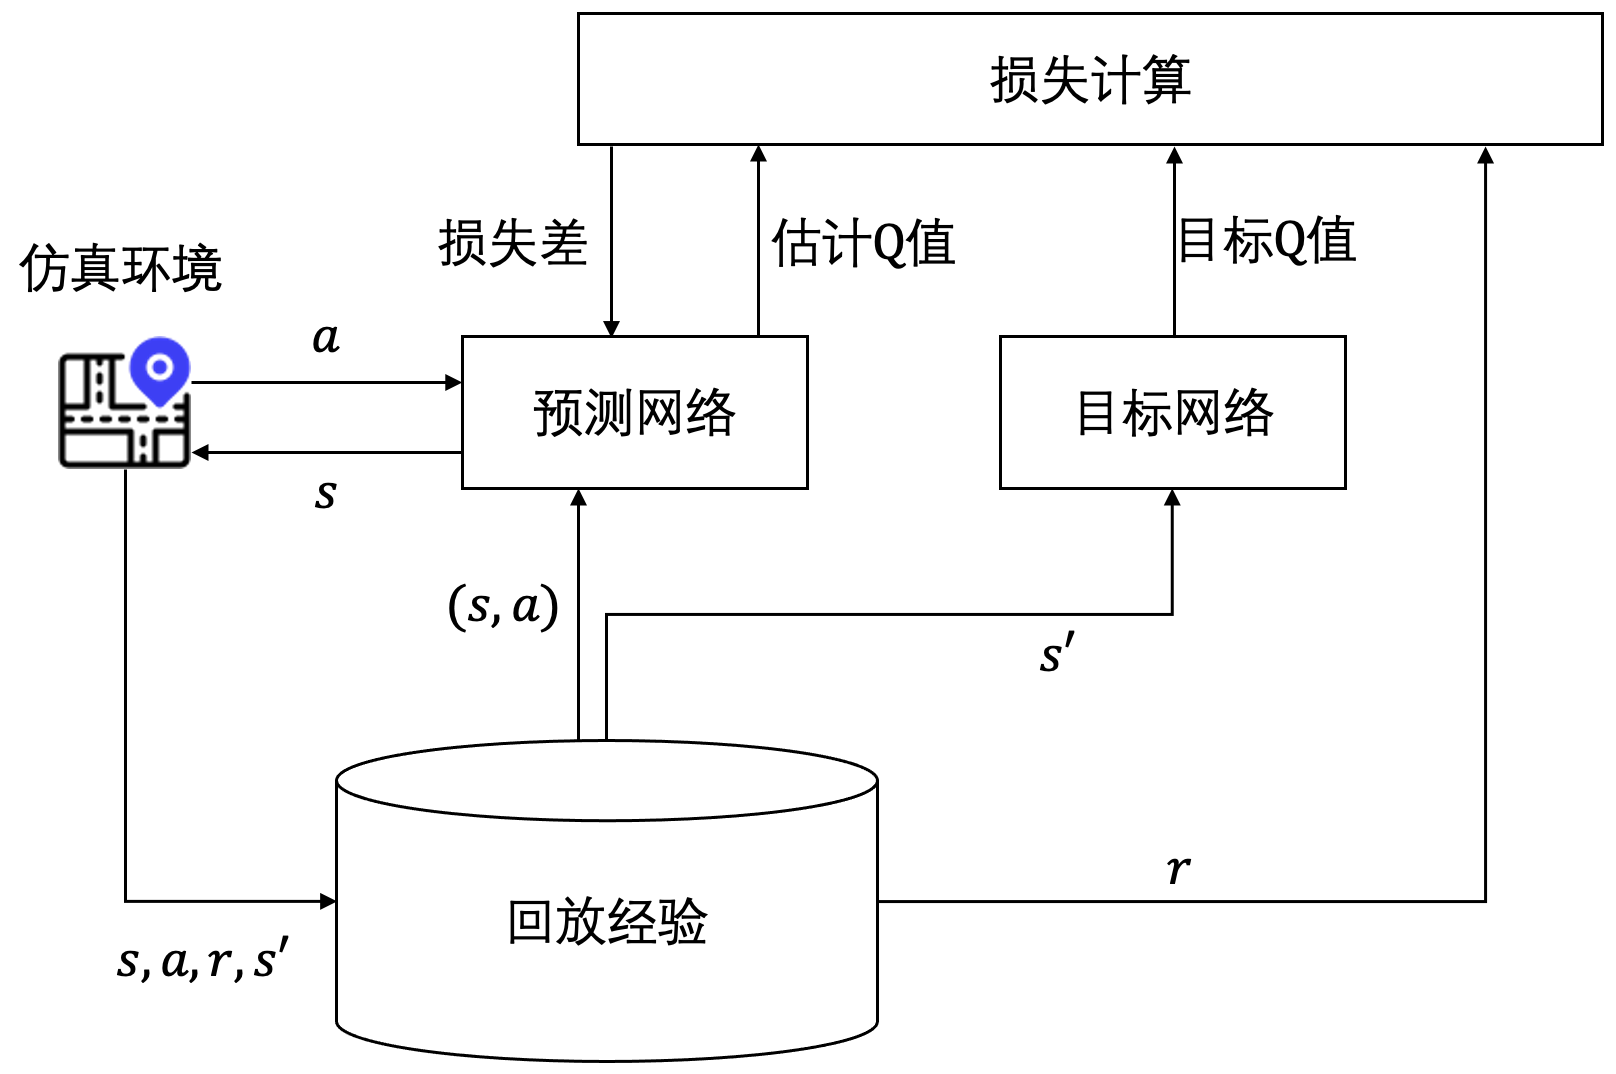
\includegraphics[width=.75\linewidth]{figures/content/reply.png}
  \caption{经验回放缓冲区的工作流程}
  \label{reply}
\end{figure}


其中,目标网络是一种防止算法中目标值剧烈变动的技术。在传统的强化学习算法中,目标值是使用当前网络计算得出的,因此目标值随着网络参数的更新而不断变化,容易导致模型不稳定。为了解决这个问题,目标网络的主要思想是使用一个独立的神经网络来计算目标值,该网络的参数较为稳定,不随着训练过程中的更新而变化。目标网络的参数定期地从当前网络中复制而来,以减缓目标值的变化速度,提高模型的稳定性。

本文的算法使用均匀随机抽样从缓冲区中选取经验元组,主要原因是打破数据间的时间相关性。在强化学习中,智能体与环境交互产生的数据序列通常具有很强的时间相关性。通过从缓冲区中均匀随机抽样,可以减小训练数据的相关性,从而减少训练过程中的不稳定性,提高模型的泛化能力和学习效率。

另一个原因是简单性和计算效率。均匀随机抽样易于实现,计算成本较低,同时可以平衡各个经验元组在训练中的使用频率。尽管优先级经验回放可能在某些情况下带来更好的性能,但其实现更复杂,涉及优先级计算、更新以及在抽样过程中的加权抽样等。因此,均匀随机抽样在许多应用中仍然是一种实用且有效的方法。在训练数据存在很大差异、关键经验对学习过程更为重要、模型收敛速度较慢或面临稀疏奖励任务时,可以考虑将均匀随机抽样改为优先级抽样。

算法\ref{DQN}是本文建立的基于深度强化学习的联合出行模式与出发时间选择建模和训练方法。算法首先初始化经验回放缓冲区和策略网络参数,然后在多个训练回合中进行迭代。在每个回合中,智能体观察初始状态,然后根据不同的时间步长确定最佳的出行模式与出发时间。接着,智能体计算总出行成本并获得相应的奖励。将观测到的经验元组存储到经验回放缓冲区,以便进行网络参数更新。最后,智能体从缓冲区中随机抽取一批样本进行学习,并定期更新目标网络参数,以提高模型的稳定性和学习效率。

\begin{algorithm}
\caption{基于深度强化学习的联合出行模式与出发时间选择建模和训练方法}\label{DQN}
\begin{algorithmic}
\State 初始化经验回放缓冲区$D$,策略网络参数$\mathbf{w}$和$\mathbf{v}$
\For{$episode = 1 \; to \; M$}
    \State 从环境中观测初始状态$s_0$
    \For{$t=1 \;  to \; T$}
        \State 使用式\ref{eq:2_22}确定时间步长为$t$时的出行模式与出发时间
        \State 根据\ref{subsection:reward}小节计算相应的总出行成本,使用式\ref{reward function}获得奖励$r_t$
        \State 记录出行和环境信息,建立下一个状态$s_{t+1}$
        \State 将元组$(\bm{s}_t,\bm{a}_t,r_t,\bm{s}_{t+1})$存储到经验回放缓冲区$D$
        \State 从$D$中随机抽取小批量样本
        \State ${Q} \leftarrow r_t + \gamma \mathop{\operatorname{argmax}}\limits_{\bm{a} \in A}\hat{q}\left(\bm{s}_{t+1}, \bm{a}, \mathbf{v}\right)$
        \State $\hat{Q} \leftarrow \hat{q}\left(\bm{s}_{t}, \bm{a}, \mathbf{w}_{t}\right)$
        \State $\mathbf{w}_{t+1} \leftarrow \mathbf{w}_{t}-\alpha \nabla \frac{1}{2}(Q-\hat{Q})^{2}$
        \State 每隔固定数量$c$个时间步,设置$\mathbf{v} \leftarrow \mathbf{w}_t$
    \EndFor
\EndFor
\end{algorithmic}
\end{algorithm}


\section{基于聚类的深度强化学习方法}
\label{sec:4_3}

在前一节中,对深度Q网络算法作为解决出行模式和时间选择问题的基本解决方案进行了详细阐述。然而,将该算法扩展为解决具有大量个体的类似问题仍然是一个挑战。正如先前讨论过的,将所有个体的经验存储并用于训练是计算上不可行且低效的,而随机选择一个或几个个体则不够准确且不可靠。因此,本节中提出了一种有效的方法来选取具有代表性的个体以进行高效的模型训练,即基于个体的出行特征进行聚类。对于处于同一聚类中的个体,可以认为它们的出行特征相似。因此,它们中的每一个都可以被视为该聚类的代表,其经验可以代表其余个体来训练深度Q网络。通过这种方式,不仅避免了部署与个体数量相同数量的代理,还有效地利用代表性个体的经验进行充分的模型训练。实际上,采用这种方法可以有效地解决具有许多个体的出行模式与时间选择问题,而在决策制定过程中不会牺牲太多的最优性。


\subsection{DBSCAN聚类方法}
密度基于空间聚类应用(Density-Based Spatial Clustering of Applications with Noise,简称DBSCAN)是一种基于密度的聚类方法,旨在识别高密度区域并将其作为簇的核心。DBSCAN的一个显著优势是无需预先确定簇的数量,因此算法本身是非参数化的。这种算法可以自适应地调整簇的大小和形状,即使在数据中存在噪声的情况下,它的性能仍然可靠。

DBSCAN算法的核心概念是将数据点划分为三类:核心点、边界点和噪声点。核心点是一个密度可达的点集,即其周围的密度大于等于指定的阈值。边界点是密度可达的点,但其周围的密度低于指定阈值。噪声点则是那些不属于任何簇的点,它们周围的密度也低于指定阈值。除了DBSCAN算法,还有其他一些聚类方法,例如k-means和层次聚类。k-means算法是一种广泛使用的聚类方法,通过将数据集划分为k个簇来实现聚类。其核心思想是将数据点分配到距离最近的质心(簇的中心),然后将质心更新为簇中所有点的平均值。接着,这一过程会不断重复,直到质心不再发生变化或达到预定的最大迭代次数为止。图\ref{pic_cluster}展示了使用DBSCAN算法的聚类效果图。


\begin{figure}
  \centering
  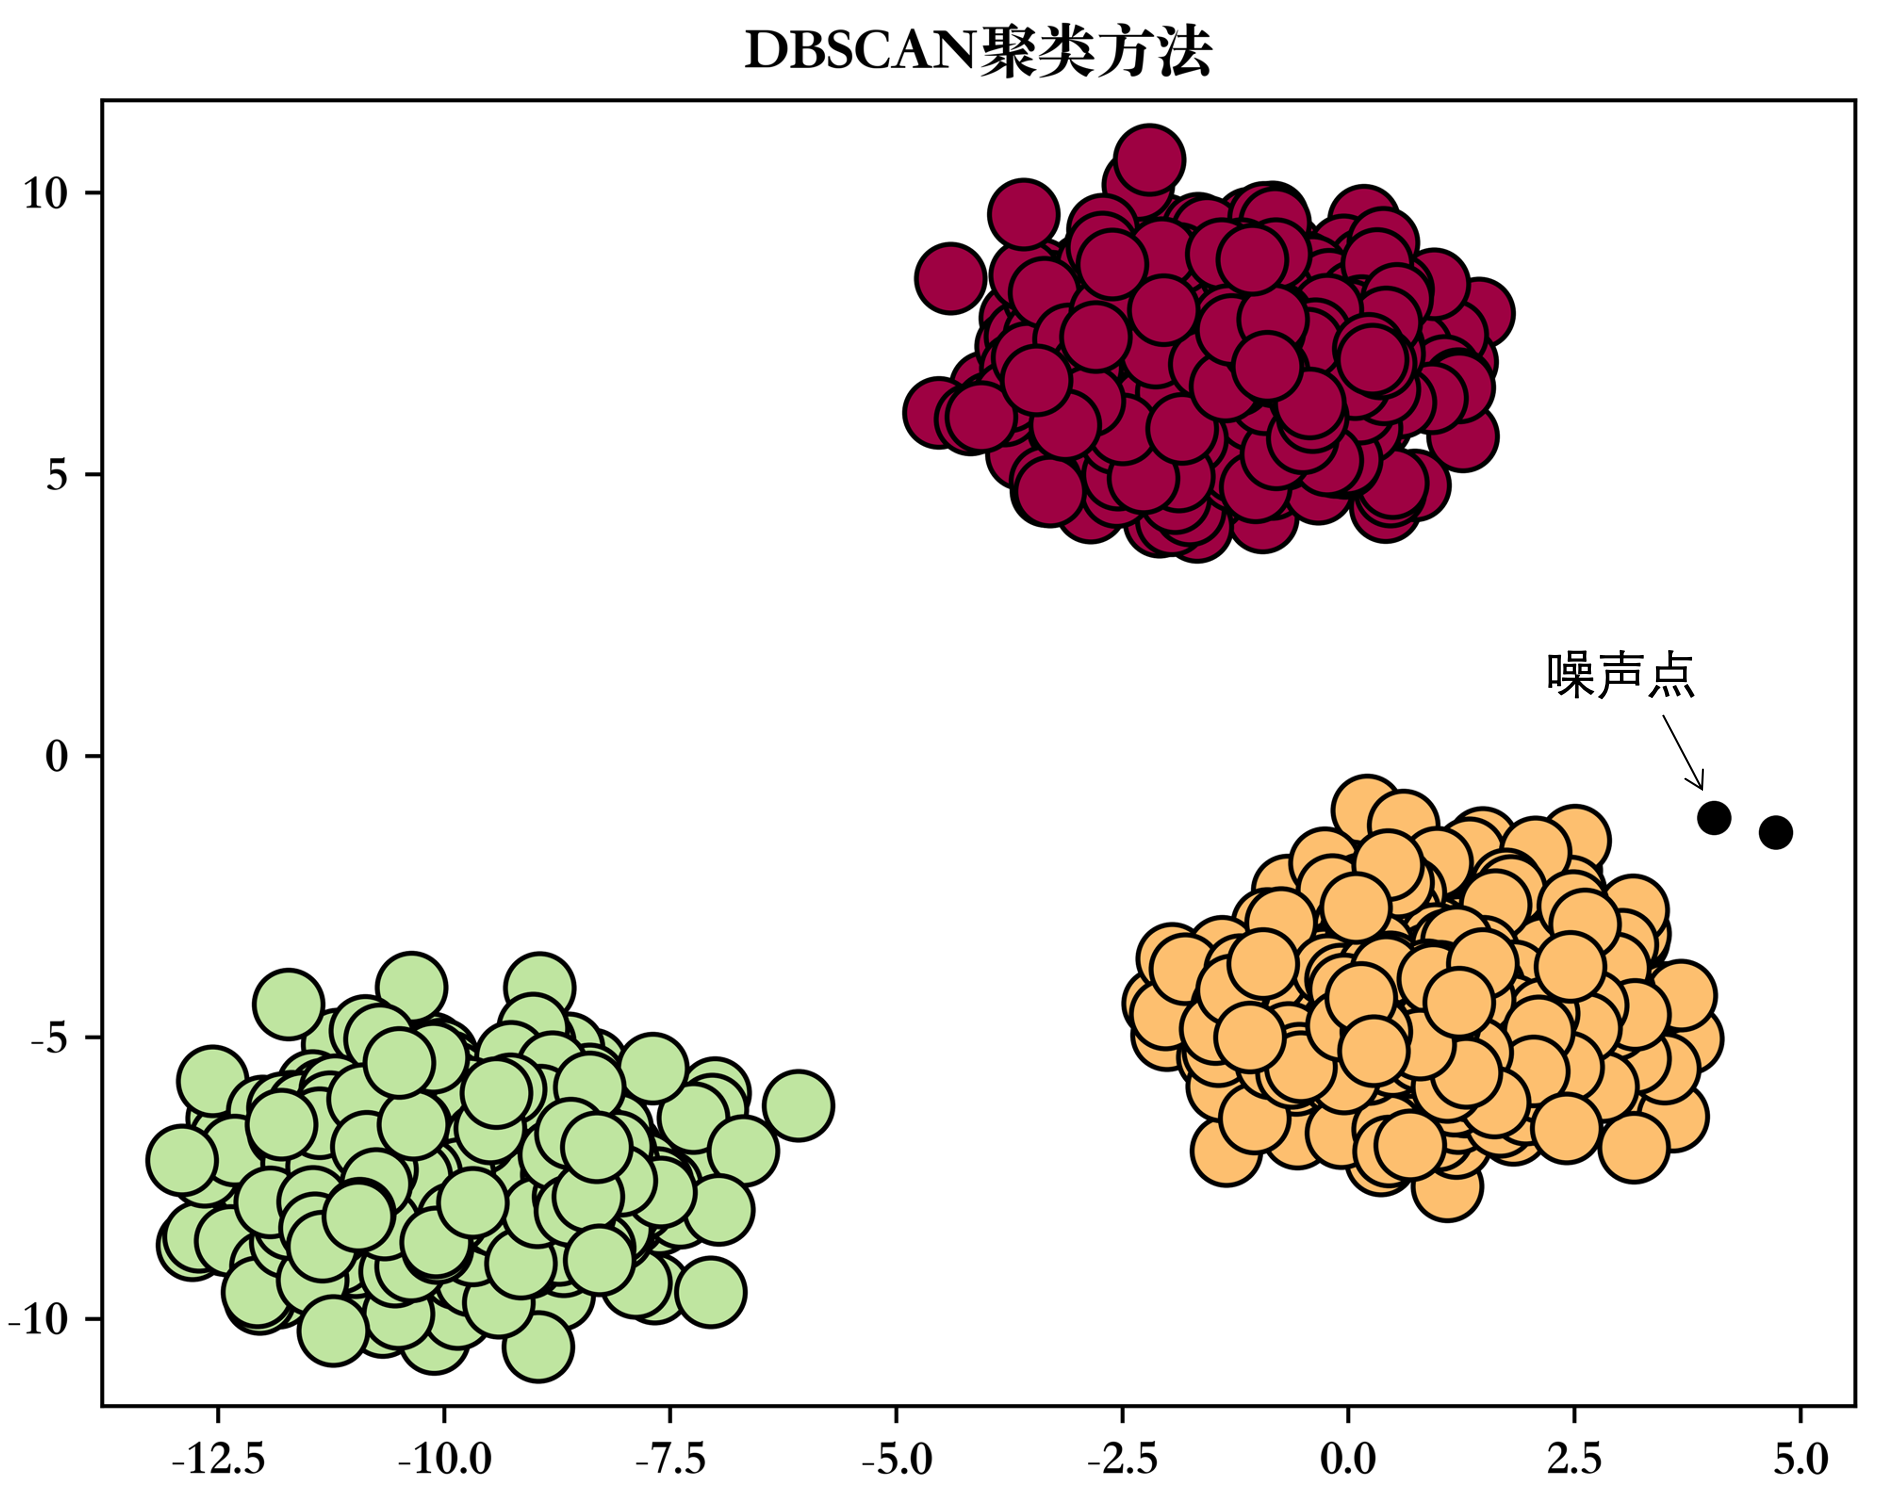
\includegraphics[width=.75\linewidth]{figures/content/cluster.png}
  \caption{DBSCAN聚类方法聚类效果图}
  \label{pic_cluster}
\end{figure}

层次聚类则是一种自下而上的聚类方法,通过递归地将最相似的数据点组合成更大的簇,最终形成一个完整的聚类树。层次聚类可以是聚合的(自底向上)或分裂的(自顶向下)。在聚合层次聚类中,每个数据点起初都是一个单独的簇,然后将最相似的簇合并在一起,直到所有数据点都被分配到一个簇中。在分裂层次聚类中,开始时将所有数据点都分配到一个大簇中,然后逐步将其分裂成较小的簇,直到达到预定的聚类数目。

尽管k-means和层次聚类方法也可以用于选择代表性个体,但它们对噪声点的处理能力不如DBSCAN,可能会将噪声点误分类为一个簇或将它们分配到多个簇中。此外,DBSCAN算法可以自动确定簇的数量,并且不需要提前指定k值或层次聚类的高度。

在这项研究中,DBSCAN算法被选作选择代表性个体的方法,因为它在处理数据噪声和密度不均匀的情况下表现出色,并且无需预先设定簇的数量。通过聚类选择代表性个体,可以显著降低强化学习算法中状态和动作空间的规模,从而提高训练效率。

总的来说,DBSCAN作为一种基于密度的聚类方法,具有很多优点。首先,它不需要预先确定簇的数量,因此更具自适应性。其次,它可以在数据中存在噪声的情况下保持较好的性能。此外,DBSCAN算法能够自动调整簇的大小和形状,使其适应不同密度的数据分布。

\subsection{聚类参数的选择}

在研究出行特征个体数据集$D$中,为了对出行数据进行有效的分类和分析,选择两个关键特征作为聚类的输入,分别是出行距离和公共交通的可达性。这两个特征在很大程度上反映了出行者的出行需求和出行方式的选择。

首先,出行距离是一个重要的出行特征,因为它与出行者的出行成本和时间成本密切相关。在现实生活中,出行距离通常会影响出行者在时间和金钱上的投入。例如,较长的出行距离可能意味着更高的燃油消耗、更多的过路费以及更长的行驶时间。此外,出行距离还与环境污染有关,较长的距离可能会导致更多的温室气体排放。因此,在对出行特征进行聚类时,出行距离是一个重要的度量标准,有助于我们了解出行者在不同距离范围内的需求和行为特征。公共交通的可达性是另一个关键特征,因为它体现了出行者对公共交通设施的依赖程度和使用意愿。在城市规划和交通管理中,公共交通的可达性对于评估城市的可持续性和交通拥堵状况具有重要意义。具有较高公共交通可达性的区域通常会吸引更多的出行者使用公共交通工具,从而减轻道路拥堵和环境污染。选择这两个特征的原因还在于它们之间可能存在的相互关系。例如,当公共交通可达性较好时,出行者可能会倾向于选择公共交通工具进行较长距离的出行,而在公共交通可达性较差的情况下,他们可能会选择私人交通工具或其他出行方式。因此,通过对这两个特征进行聚类,可以揭示出行者在不同场景下的出行偏好和需求。此外,在实际应用中,出行距离和公共交通可达性还可以与其他出行特征相结合,以提供更全面的出行数据分析。例如,可以结合出行者的年龄、职业、家庭状况等社会经济特征,以深入了解不同人群在出行距离和公共交通可达性方面的需求和偏好。这将有助于城市规划者和交通管理者制定更有效的交通政策和措施,以满足不同人群的出行需求。


\subsection{深度强化学习模型的改进}
通过将深度强化学习方法与个体聚类和获取代表智能体的过程相结合,该集成算法旨在解决具有多个体的出行模式与时间选择问题。在这种方法中,所需训练的代理数量等于选定的代表智能体数量,从而降低了计算复杂度和训练时间。在整个训练过程中,这些代表智能体与它们各自的经验存储池同时进行训练。在训练的过程中,代表智能体学习并优化它们在出行场景中的决策。当这些代表智能体经过充分训练后联合起来,为不同的个体提供出行选择决策,从而提高整体系统的效率和性能。这种集成算法的优势在于一旦代表智能体训练完成,就无需重新进行聚类,因为它们已经具备了为聚类中各个个体做出决策的能力。在实际应用中,这些代表智能体将评估可用的出行选项,并选择具有最高奖励的行动来实施。这种方法有助于确保个体能够在各种出行场景中作出合理且有效的决策,从而提高整体系统的性能。

算法\ref{DBSCAN}用于聚类个体并获取代表智能体。给定一组具有出行特征的个体数据集$D$、距离阈值$\mu$和形成聚类所需的最小点数$m$,算法首先对数据进行归一化,然后遍历每个非聚类个体。对于每个个体$\bm{x}$,算法计算其在阈值$\mu$内的邻居集$N$。如果邻居集的大小小于$m$,则将个体$\bm{x}$标记为噪声;否则,将其设置为新聚类$C$的核心点。接着,算法遍历$N$中的每个个体,并更新邻居集和聚类。最终,算法返回用于获取代表的个体群集。

算法\ref{DBSCAN}实现了DBSCAN聚类过程,用于处理具有出行特征的个体数据集。通过这种方式,算法能够将个体划分为不同的聚类,同时识别并处理噪声点,从而在聚类中找到具有代表性的个体。

\begin{algorithm}
\small
\caption{聚类个体并获取代表智能体}\label{DBSCAN}
\begin{algorithmic}
\Require   所有个体的出行特征$D=\left\{\bm{x}_{1}=[L_{1}, p_{1}]^T, \bm{x}_{2}, \ldots, \bm{x}_{m}\right\}$,距离阈值$\mu$,形成聚类所需的最小点数$m$
\Ensure 代表智能体的集群
\State 数据归一化:$x_{\text {normalized }}=\frac{x-x_{\min }}{x_{\max }-x_{\min }}$
\For{每个非聚类个体 $\bm{x} \in D_{\text {normalized }}$}
    \State 将个体$\bm{x}$标记为归入某个群组
    \State $N \leftarrow GetNeighbors(\bm{x},\mu)$
    \If{$|N| < m$}
        \State 将个体$\bm{x}$标记为噪声
    \Else
        \State 设置新聚类$C \leftarrow {\bm{x}}$
        \For{每个个体 $\bm{x'} \in N$}
            \State $N \leftarrow N \backslash \bm{x'}$
            \If{个体$\bm{x'}$是非聚类的}
                \State 将个体$\bm{x'}$标记为已聚类
                \State $N' \leftarrow GetNeighbors(\bm{x'},\mu)$
                \If{$|N'| \geq m$}
                    \State $N \leftarrow N \cup N'$
                \EndIf
                \If{$\bm{x'}$是噪声}
                    \State $C \leftarrow C \cup \{ \bm{x'} \}$
                \EndIf
            \EndIf
        \EndFor
    \EndIf
\EndFor
\end{algorithmic}
\end{algorithm}

\section{本章小结}

本章主要介绍了基于深度强化学习的出行模式与时间选择方法。首先,在\ref{sec:4_1}节中建立了马尔可夫决策过程框架,定义动作空间、状态空间和奖励函数。接下来,在\ref{sec:4_2}节中采用基于深度神经网络的算法,设计了神经网络结构,并通过选择合适的超参数和优化模型来改善出行模式与出发时间选择的准确性。为了进一步提高算法性能,本章在\ref{sec:4_3}节中还引入了基于聚类的深度强化学习方法。通过使用合适的聚类方法和参数选择,对出行数据进行了预处理,以便在深度强化学习模型中实现更好的特征提取和泛化能力。最后,通过对深度强化学习模型进行改进,提高了出行模式与时间选择的准确性和稳定性。
